\section{Datenvorverarbeitung}
\label{subsec:revpar_prepare}
Die Datenvorverarbeitung dient dazu, zu ermitteln, welche Daten bereits vorhanden sind und wie sie modifiziert werden müssen, um die Entwicklung eines generellen Modells zu ermöglichen.
\newpage
\begin{figure}[h]
    \centering
    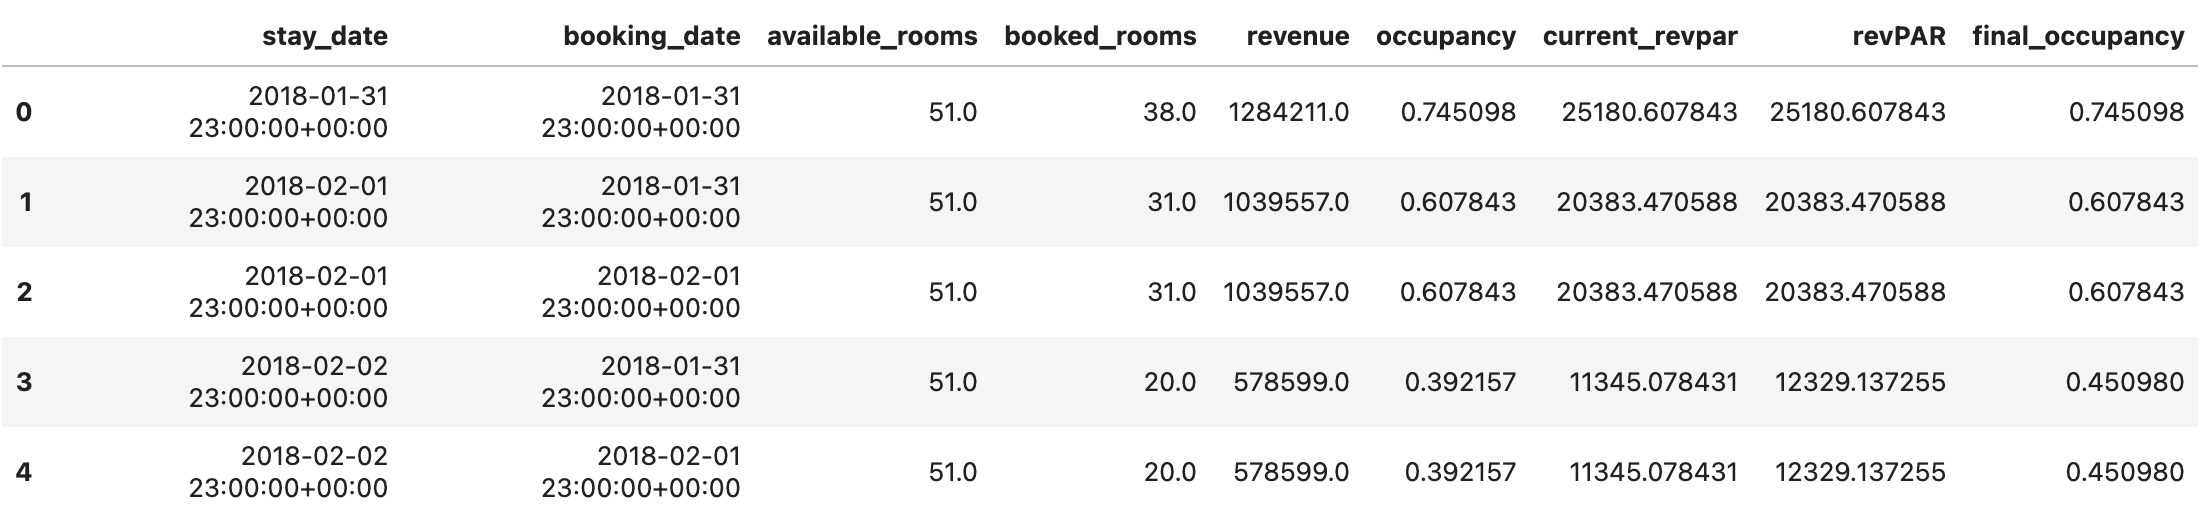
\includegraphics[width=1\textwidth, center]{revpar_features.png}
    \caption[Bereits vorhandene Hotelspezifischen Daten]{Bereits vorhandene Hotelspezifischen Daten}
    \label{img:revpar_features}
\end{figure}

Abbildung \ref{img:revpar_features} veranschaulicht beispielhaft die Vergangenheitsdaten, wie sie aus der Datenbank abgerufen werden können. Dabei repräsentiert die Spalte \emph{revPAR} den zu prognostizierenden Wert. Es ist zu erkennen, dass diese Werte sich spezifisch auf das ausgewählte Hotel beziehen und daher in ihrer aktuellen Form nicht für das Training verwendet werden können. Die vorgeschlagene Vorgehensweise besteht darin, sämtliche hotelspezifischen Spalten durch den Durchschnittswert der jeweiligen Spalte zu skalieren, um einen standardisierten Wert zu erlangen, der für jedes Hotel verwendet werden kann.
\newline 
\newline
Im Folgenden werden mehrere Funktionen definiert, die einerseits weitere Daten zum Datensatz hinzufügen sollen und andererseits die vorhandenen Spalten, wie oben beschrieben, durch den Durchschnittswert normieren sollen:

\begin{lstlisting}[language=Python, label=lst:revpar_helper_funcs, caption=Hilfsfunktions für das RevPAR Modell]
# list holiday
list_holidays = ['holiday_Neujahr', 'holiday_Christi Himmelfahrt','holiday_Erster Mai',
               'holiday_Karfreitag', 'holiday_Ostermontag','holiday_Pfingstmontag',
                 'holiday_Tag der Deutschen Einheit', 'holiday_Reformationstag', 'holiday_Erster Weihnachtstag', 
                 'holiday_Zweiter Weihnachtstag', 
                 ]

# list months
list_months = ['start_date_monthName_January', 'start_date_monthName_February', 'start_date_monthName_March', 
               'start_date_monthName_April', 'start_date_monthName_May', 'start_date_monthName_June',
               'start_date_monthName_July', 'start_date_monthName_August', 'start_date_monthName_September', 
               'start_date_monthName_October', 'start_date_monthName_November', 'start_date_monthName_December' ]

# list days
list_days = ['start_date_weekDayName_Monday', 'start_date_weekDayName_Tuesday', 'start_date_weekDayName_Wednesday',
            'start_date_weekDayName_Thursday', 'start_date_weekDayName_Friday', 'start_date_weekDayName_Saturday', 
             'start_date_weekDayName_Sunday']

# Vorbereiten der Hotelfeatures
def add_holidays_as_bool(df):
    ger_holidays = holidays.Germany()
    df['holiday'] = df.stay_date.apply(lambda x: ger_holidays.get(x.date()))
    df['holiday'] = df['holiday'].notnull().astype(int)
    return df

def add_month_feature(df):
    df.insert(loc=1, column='stay_date_monthName', value=df['stay_date'].dt.month_name())  
    return df

def add_weekDay_feature(df):
    df.insert(loc=1, column='stay_date_weekDayName', value=df['stay_date'].dt.day_name())
    return df

def add_year(df):
    df.insert(loc=1, column='stay_date_year', value=df['stay_date'].dt.year)
    return df

def feature_ADR(df):
    df['ADR'] = df['revenue'] / df['booked_rooms']
    df.loc[df['booked_rooms'] == 0, 'ADR'] = 0
    
    durchschnitt = np.mean(df['ADR'])
    df["scaled_current_adr"] = df['ADR'] / durchschnitt

    return df

def add_time_to_arrival(df):
    df['time_to_arrival'] = df['stay_date'] - df['booking_date']
    df['time_to_arrival'] = df['time_to_arrival'].dt.days
    return df

def add_stay_date_str(df):
    df["stay_date_str"] = df["stay_date"].dt.strftime("%d.%m.%Y")
    return df

def add_scaled_revpar_values(df):
    durchschnitt = np.mean(df['revPAR'])
    df["target"] = df['revPAR'] / durchschnitt
    df["scaled_current_revpar"] = df['current_revpar'] / durchschnitt
    return df
\end{lstlisting}

\begin{figure}[h]
    \centering
    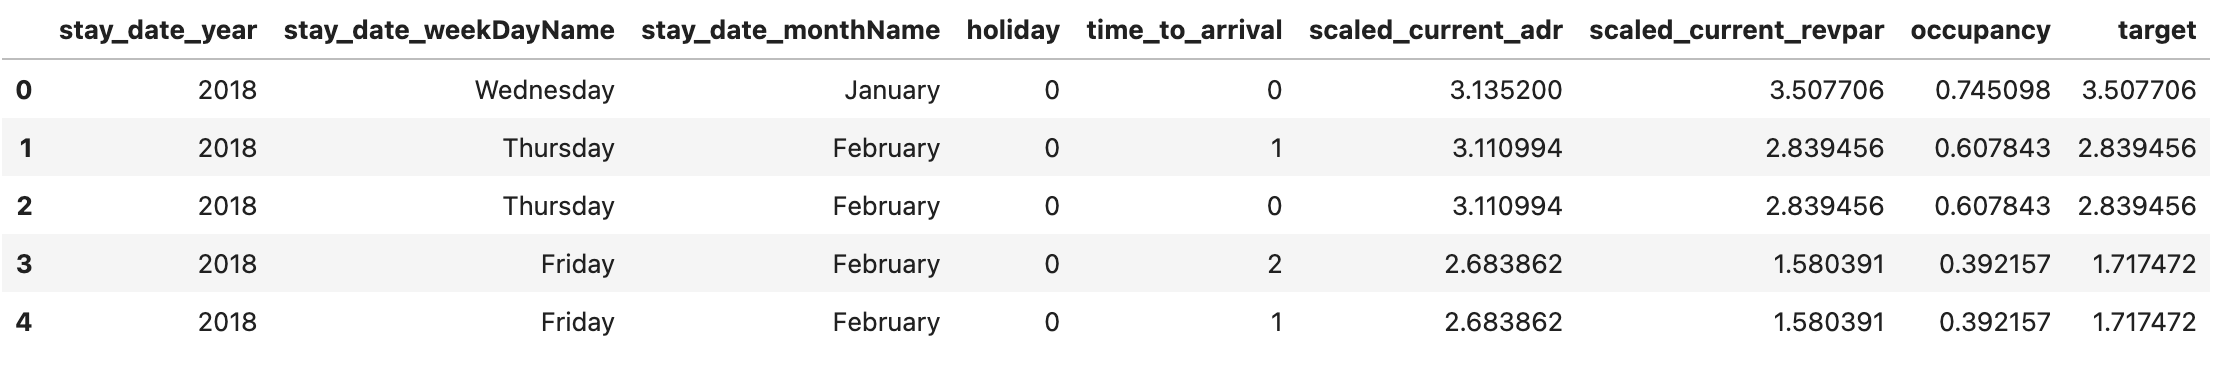
\includegraphics[width=1\textwidth, center]{revpar_features_2.png}
    \caption[Datensatz nach der Ausführung der Hilfsfunktionen]{Datensatz nach der Ausführung der Hilfsfunktionen}
    \label{img:revpar_features_2}
\end{figure}

Abbildung \ref{img:revpar_features_2} zeigt den Datensatz nach der Ausführung der Funktionen in Listing \ref{lst:revpar_helper_funcs}. Es ist zu erkennen, dass der Datensatz nun ausschließlich normierte Werte enthält. Im Folgenden wird eine Datenanalyse auf diesem Datensatz durchgeführt.
